\documentclass[fr]{../../../../../../eplexam}

\usepackage{../../../../../../eplunits}

\hypertitle[']{Optique et lasers}{7}{PHYS}{2143}{2019}{Janvier}{All}
{Olivier Leblanc}
{Alain Cornet et Clément Lauzin}

Examen de 4h à 4 questions, où on demande de choisir seulement 3 questions auxquelles répondre.
Un formulaire manuscrit recto-verso format A4 est autorisé.

\section{}

\subsection*{Partie I}

Contexte : Nous voulons étudier l'existence de mirages. Dans un désert chaud, l'indice de réfraction varie avec la hauteur selon une loi :

\[
    n^2(z) = az+b
\]

On pose K tel que : $n_0 \sin(i_0) = \frac{1}{\sqrt{K}}$.

\begin{figure}[h!]
    \centering
    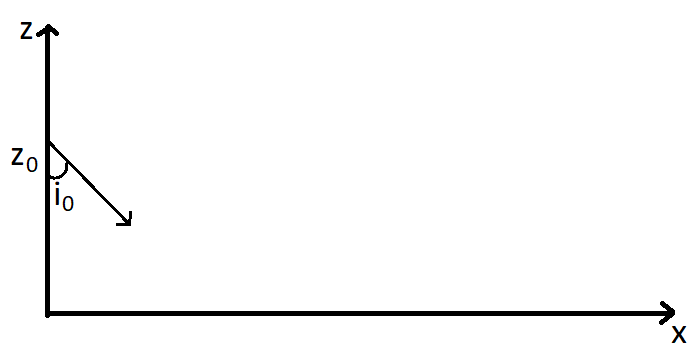
\includegraphics[scale=0.6]{02.png}
    \caption{}
    \label{}
\end{figure}

\begin{enumerate}
 \item Rappeler l'équation différentielle des rayons lumineux.
 \item Montrer que la trajectoire peut s'écrire :
    \[
    z = \frac{aK}{4} x^2 + \frac{\cos(i_0)}{\sin(i_0) x + z_0}
    \]
 \item Expliquer la forme de la trajectoire. Quelle est sa concavité ?
 \item Justifier l'existence des mirages en s'aidant d'un schéma.
\end{enumerate}

\subsection*{Partie II}

On désire former un rayon lumineux qui se propage entre deux plans horizontaux espacés d'une hauteur a selon une loi sinusoïdale : $ z = \mathrm{asin}(bx) $.

Montrez que l'expression de l'indice de réfraction du milieu (ne dépendant que de z) peut s'écrire : 
\[
    n(z) = n_0 \sqrt{1 - \frac{b^2}{1+a^2b^2}z^2}
\]


\begin{solution}
 
 \subsection*{Partie I}
 
 \begin{enumerate}
  \item \begin{center}
            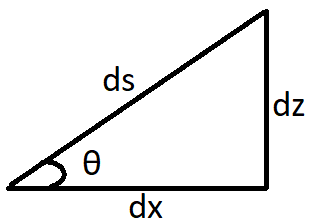
\includegraphics[scale=0.3]{01.png}
        \end{center}

    La loi de Snell-Descartes donne : $$n_0\sin(i_0) = \frac{1}{\sqrt{K}} = n(z) \cos(\theta)$$
    De plus, on a : 
    \[
        \sin(\theta)^2 + \cos(\theta)^2 = 1 \Leftrightarrow \cos(\theta) = \frac{1}{\sqrt{1+\tan(\theta)^2}} = \frac{1}{\sqrt{1+(\frac{dz}{dx})^2}}
    \]

    Donc, l'équation différentielle des rayons est : 

    \[
        \frac{1}{\sqrt{K}} = \frac{n(z)}{\sqrt{1+(\frac{dz}{dx})^2}}
    \]
  \item On intègre l'équation différentielle en tenant compte de l'expression donnée de n(z) : 
    \[
        \frac{1}{\sqrt{K}} = \frac{n(z)}{\sqrt{1+(\frac{dz}{dx})^2}}  \Leftrightarrow (aK)z+(bK) = 1 + (\frac{dz}{dx})^2  \Leftrightarrow \left[(aK)z + (bK-1)\right]^{\frac{-1}{2}} dz = dx
    \]
    \[
        \Leftrightarrow \frac{2[(aK)z + (bK-1)]^{\frac{1}{2}}}{(aK)} = x + C
    \]
    \[
    \Leftrightarrow (aK)z + (bK-1) = \left( \frac{(aK)x}{2} + C' \right) ^2 = \frac{(aK)^2}{4}x^2 + (aK)C'x + C'^2 \Leftrightarrow z = \frac{(aK)}{4} x^2 + C'x + z_0 
    \]

    Avec la condition limite : $ \frac{dz}{dx} (x=0) = \frac{1}{\tan(i_0)} = C'$ (voir dessin), on retombe sur l'expression de l'énoncé.
  \item La trajectoire est une parabole orientée vers le haut (car $\frac{(aK)}{4}$ est positif).
  \item \nosubsolution
 \end{enumerate}
 
 \subsection*{Partie II}

 On reprend l'équation différentielle des rayons : $$C = \frac{n(z)}{\sqrt{1+(\frac{dz}{dx})^2}} $$ et on résoud pour $n(z)$. Avec $\frac{dz}{dx} = ab \cos(bx) = ab \cos(\mathrm{asin}(\frac{z}{a})) = ab \sqrt{1- (\frac{z}{a})^2}$.
 En posant $n_0 = C \sqrt{1+a^2b^2}$, on obtient l'expression voulue.
 
\end{solution}

\section{}

\begin{figure}[h!]
    \centering
    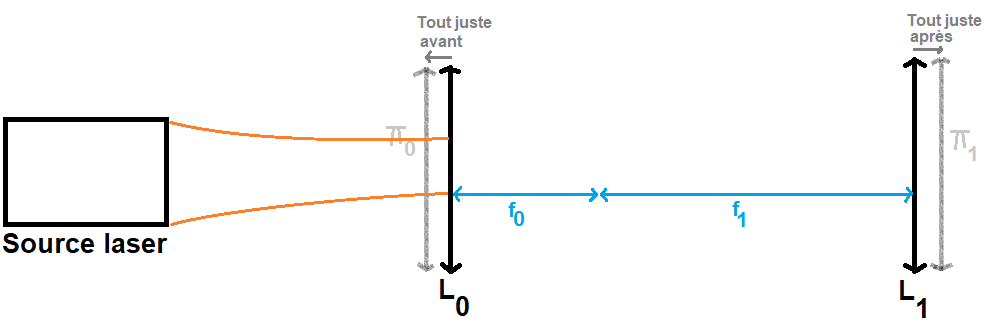
\includegraphics[width=0.8\textwidth]{ex4.png}
    \caption{Montage expérimental}
    \label{ex4}
\end{figure}

Le système décrit par la figure \ref{ex4} est un essai pour réduire la divergence d'un laser. On a le waist $w_0$ à la lentille $L_0$. $z_R$ est donné. La longueur d'onde du laser formé est $\lambda_0 = \SI{532}{nm}$.

\begin{enumerate}
    \item Dans quelle gamme de couleur est le rayon?
    
    \item Exprimer $w_0$ et $\theta$ en fonction de $z_R$.
    
    
    \item Faire l'application numérique pour $z_R = \SI{10}{cm}$.
    
    \item 
    
    \begin{enumerate}
     \item Trouver $T_{\Pi_0 \rightarrow \Pi_1}$, la matrice de transfert. Vérifier que $C=0$ et $A\cdot D$ a la valeur attendue.
     \item Soit $q_0$ et $q_1$ les rayons de courbure complexe en $\Pi_0$ et $\Pi_1$. Exprimer $q_0$ en fonction des données du problème. Exprimer $q_1$ en fonction de $f_0$, $f_1$ et $q_0$, puis ensuite $f_0$, $f_1$ et $z_R$. 
     \item Soit $O"$ la position du waist après transformation par le système optique. Rappeler $q_1(q")$ et $\overline{O"\Omega_1}$. Par identification, donner $z_R"$ et  $\overline{O"\Omega_1}$. Le waist se trouve-t-il à gauche ou à droite de $L_1$?
     \item Exprimer le nouvel angle de divergence. Quelle est la condition pour avoir réduction de la divergence? Quel est le facteur? 
     \item Que peut-on dire du nouveau waist $w_0 "$? 
     \item Bonus : Trouver $f_0$ et $f_1$ pour obtenir un waist de \SI{2.2}{m} après $L_1$ et réduction de 10.
    \end{enumerate}
    
\end{enumerate}

\begin{solution}

\begin{enumerate}
    \item Visible (bleu-vert).
    \item $w_0 = \sqrt{\frac{\lambda z_R}{\pi}}$ \hspace{3cm} $\theta = \mathrm{atan} \left( \frac{\lambda}{\pi w_0} \right) \approx \frac{\lambda}{\pi w_0} $.
    \item $w_0 = \SI{130}{\micro m}$ et $\theta \approx \SI{1.3e-3}{rad}$.
    \item 
    
    \begin{enumerate}
     \item $T_{\Pi_0 \Rightarrow \Pi_1} = T_{L_1}.T_{propag}.T_{L_0} 
        = \begin{bmatrix} 1 & 0 \\ \frac{-1}{f_1} & 1 \\ \end{bmatrix} 
        = \begin{bmatrix} 1 & f_0+f_1 \\ 0 & 1 \\ \end{bmatrix} 
        = \begin{bmatrix} 1 & 0 \\ \frac{-1}{f_0} & 1 \\ \end{bmatrix}
        = \begin{bmatrix} \frac{-f_0}{f_1} & f_0+f_1 \\ 0 & \frac{-f_1}{f_0} \\ \end{bmatrix}$
        $A\cdot D=1$ comme attendu car on reste dans le même milieu, il n'y a donc pas de changement d'indice de réfraction. 
     \item $q_0 = i.z_R$. On a $r_i=w_i$ et $\theta_i = \frac{w_i}{q_i}$. On applique la matrice $\begin{bmatrix} w_1  \\ \frac{w_1}{q_1}  \\ \end{bmatrix}
        = T_{\Pi_0 \Rightarrow \Pi_1}.\begin{bmatrix} w_0  \\ \frac{w_0}{q_0}  \\ \end{bmatrix}$. \\
        On trouve $q_1 = \left( \frac{f_1}{f_0} \right)^2q_0 - (f_1+f_0) \frac{f_1}{f_0} = i  \left( \frac{f_1}{f_0} \right)^2z_R -  (f_1+f_0) \frac{f_1}{f_0}$. 
     \item $q" = q_1 + \overline{O"\Omega_1} \Leftrightarrow q_1 = iz_R + \overline{O"\Omega_1} = i  \left( \frac{f_1}{f_0} \right)^2z_R \underbrace{- (f_1+f_0) \frac{f_1}{f_0}}_{<0 \text{ donc à gauche de } L_1}$ 
     \item $\theta^" = \frac{w"}{q"}=\frac{w_1}{q_1} = \frac{-f_1}{f_0} \frac{w_0}{q_0} = \frac{-f_1}{f_0} \theta$. La condition pour avoir réduction de divergence est donc $f_1>f_0$.
     \item $|w_0"| = \frac{f_1}{f_0} |w_0|$. Le nouveau waist est plus large. Ce qui est logique car plus un faisceau est large, moins il est divergent.
     \item Bonus: $f_1 = 10(-f_0)$ avec $f_1=\SI{244}{mm}$.
    \end{enumerate}
    
\end{enumerate}

\end{solution}

\end{document}


